% \text{mA}in.tex
\documentclass{Report} % 使用您自定义的类

% --- 设置所有封面和页眉的占位符信息 ---
\ReportLogo{ZJU.jpg} % 您的代码指定了 ZJU.jpg
\Major{信息工程}
\StudentName{何~铭~源}
\StudentID{3240104481}
\ReportDate{\today}
\ReportLocation{紫金港东四219}

\CourseName{电子电路设计实验I}
\TeacherName{施红军、叶险峰、邓靖靖}
\ExperimentName{叠加定理实验研究} % 此项也会用于页眉
\ExperimentType{验证类实验}
\TeamMate{孙潇枫}
\newcolumntype{C}{>{\centering\arraybackslash}c}
\usepackage{tabularx}
\usepackage{subcaption}
\begin{document}


\makecover

\section{实验目标}
本实验旨在实现以下两个主要目标：
\begin{itemize}
    \item 通过实验操作，深入探究并理解戴维南定理的核心内容。
    \item 学习并掌握测量一个有源二端口网络等效电路参数（如等效电压和等效电阻）的具体方法。
\end{itemize}

\section{实验内容与要求}
本实验的任务和具体要求如下：
\begin{itemize}
    \item 实际测量用于验证戴维南定理的各项关键等效参数，主要包括网络的开路电压（$U_{OC}$）和短路电流（$I_{SC}$）。
    \item 运用测量得到的参数，动手构建出相应的等效电路模型，并基于此模型对戴维南定理的准确性进行实验验证。
\end{itemize}

\section{理论基础}
戴维南定理是电路分析中的一个重要原理。它指出，对于任何一个线性网络，当我们只关注其中某一条支路的电压与电流时，可以将电路的其余部分（无论其内部多么复杂）简化并视为一个含源的单端口网络。这个等效的单端口网络可以进一步被模型化为一个理想电压源和一个电阻的串联。

具体来说，如果将这个含源网络等效为一个电压源模型：
\begin{itemize}
    \item \textbf{等效电压源：} 其电压源的电动势 $U_s$（或 $U_{OC}$）等于原网络在该端口处的开路电压。
    \item \textbf{等效内阻：} 其等效电阻 $R_o$ 等于将原网络中所有独立的电源均置零（即所有理想电压源视为短路，所有理想电流源视为开路）后，从该端口看进去的输入电阻。
\end{itemize}
这个由等效电压源 $U_s$ 和等效电阻 $R_o$ 串联组成的电路，就是原网络的戴维南等效电路。




\section{实验方案设计与参数计算}
\subsection{实验方案总体设计}
\begin{figure}[H]
\centering
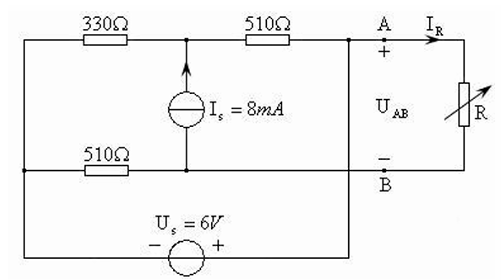
\includegraphics[width=0.6\textwidth]{./fig/戴维南.png}
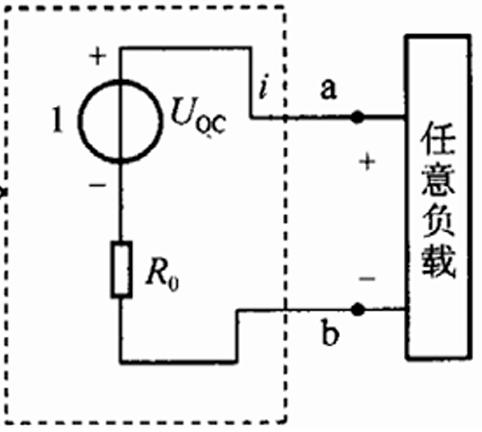
\includegraphics[width=0.6\textwidth]{./fig/戴维南等效.png}
\caption{设计电路验证原电路和其戴维南等效电路的伏安特性曲线}\label{fig}
\end{figure}
本次实验的核心目的是利用\cref{fig}所示的电路，来对戴维南等效进行实验验证，并探究其适用范围。

\begin{enumerate}
    \item \textbf{测量等效参数：} 采用“开路电压法”和“短路电流法”相结合的方式，对原始的有源二端口网络进行测试，以确定其戴维南等效电路的两个关键参数：等效电动势 $U_{OC}$ 和等效内阻 $R_O$。

    \item \textbf{测试原网络外特性：} 搭建原始电路，在输出端口接入一个可变负载电阻 $R_L$。通过多次改变 $R_L$ 的阻值，测量并记录一系列对应的电阻大小，端口电压和电流值，以此来描绘原网络的外特性曲线。

    \item \textbf{搭建等效电路并验证：}
    \begin{itemize}
        \item \textbf{构建等效电路：} 按照实验电路，构建戴维南等效模型。使用一个直流稳压电源模拟等效电动势 $U_{OC}$。使用一个电位器来模拟等效内阻 $R_O$，并将其阻值精确调整至步骤 (1) 中测得的 $R_O$ 值。
        \item \textbf{测试与比较：} 在搭建好的等效电路上，重复步骤 (2) 中的负载实验，即接入相同的可变负载 $R_L$，测量并记录其外特性数据。
        \item \textbf{分析验证：} 将原网络的外特性数据与等效电路的外特性数据进行对比。如果两者在允许的误差范围内基本一致，即可验证戴维南定理的正确性。
    \end{itemize}
\end{enumerate}


\subsection{理论值计算}

\subsection{开路电压}

\begin{figure}[H]
\centering
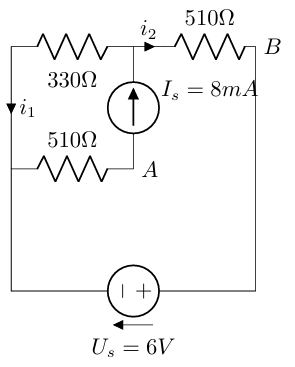
\includegraphics[width=0.4\textwidth]{./fig/开路.png}
\caption{开路电路}
\label{fig:op}
\end{figure}

如\cref{fig:op}，画出 A 和 B 开路时的等效电路：
\begin{equation}
\Rightarrow U_{AB} = 6 + (510 \cdot I_s) = 10.08V
\end{equation}

\subsection{短路电流}

\begin{figure}[H]
\centering
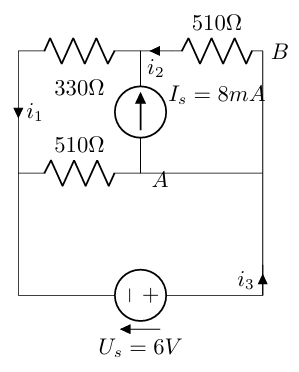
\includegraphics[width=0.4\textwidth]{./fig/短路.png}
\caption{短路电路}
\label{fig:sc}
\end{figure}

利用网孔电流法：
\begin{equation}
\begin{cases}
    840i_1 + 510i_2 - 510i_3 = 0 \\
    i_1 - i_2 = I_s \\
    510(i_3 - i_1) = 6
\end{cases}
\end{equation}

解得：
\begin{equation}
\begin{cases}
    i_1 = 12.4\text{mA} \\
    i_2 = 4.44\text{mA} \\
    i_3 = 24.209\text{mA}
\end{cases}
\end{equation}

短路电流即 AB 间的电流
\begin{equation}
    I_s = i_3 - i_2 = 19.77\text{mA}
\end{equation}

\section{实验仪器设备}
\begin{itemize}
    \item 万用表
    \item 电流表
    \item 实验室提供的电路板
\end{itemize}


\section{实验步骤、实验数据记录}

\subsection{原电路}
用开路电压、短路电流法测定戴维南等效电路的 $U_{OC}$、$R_O$ 和诺顿等效电路的 $I_{SC}$、$R_O$。接入稳压电源 $U_s = 6V$ 和恒流源 $I_s = 8mA$，接入负载 $R_L$。测出 $U_{OC}$ 和 $I_{SC}$，并计算出 $R_O$。

%
% 表 1：实验数据
% 我已将 (10.24, 19.57, 523.25) 替换为您提供的 (10.13, 19.22, 527.06)
%
\begin{table}[H]
    \centering
    \caption{实验数据}
    \label{tab:data1}
    \begin{tabular}{ccc}
        \toprule
        $U_{OC} \text{(V)}$ & $I_{SC} \text{(mA)}$ & $R_O = U_{OC} / I_{SC} (\Omega)$ \\
        \midrule
        10.13 & 19.22 & 527.06 \\
        \bottomrule
    \end{tabular}
\end{table}

% (2)
接入负载 $R_L$，改变 $R_L$ 阻值，测量有源二端口网络的外特性，实验数据如下：

%
% 表 2：负载实验数据
% 我已将图片中的数据替换为您提供的新数据
%
\begin{table}[H]
    \centering
    \caption{记录九组原电路的伏安特性曲线} % 原图无标题
    \begin{tabular}{lccccccccc}
        \toprule
         & 1 & 2 & 3 & 4 & 5 & 6 & 7 & 8 & 9 \\
        \midrule
        $R_L (\Omega)$ & 4.5 & 48.4 & 119.8 & 239 & 277 & 335 & 418 & 644 & 790 \\
        $U_{AB} \text{(V)}$ & 0.08 & 0.68 & 1.98 & 3.55 & 4.03 & 4.59 & 5.37 & 7.02 & 7.86 \\
        $I \text{ (mA)}$ & 19.12 & 17.87 & 15.43 & 12.33 & 11.56 & 10.42 & 9.06 & 5.87 & 4.27 \\
        \bottomrule
    \end{tabular}
\end{table}
\section{数据分析与讨论}
    使用Origin拟合两个电路的伏安特性曲线
    \begin{figure}[H]
    \centering
    \begin{subfigure}[b]{0.45\textwidth}
        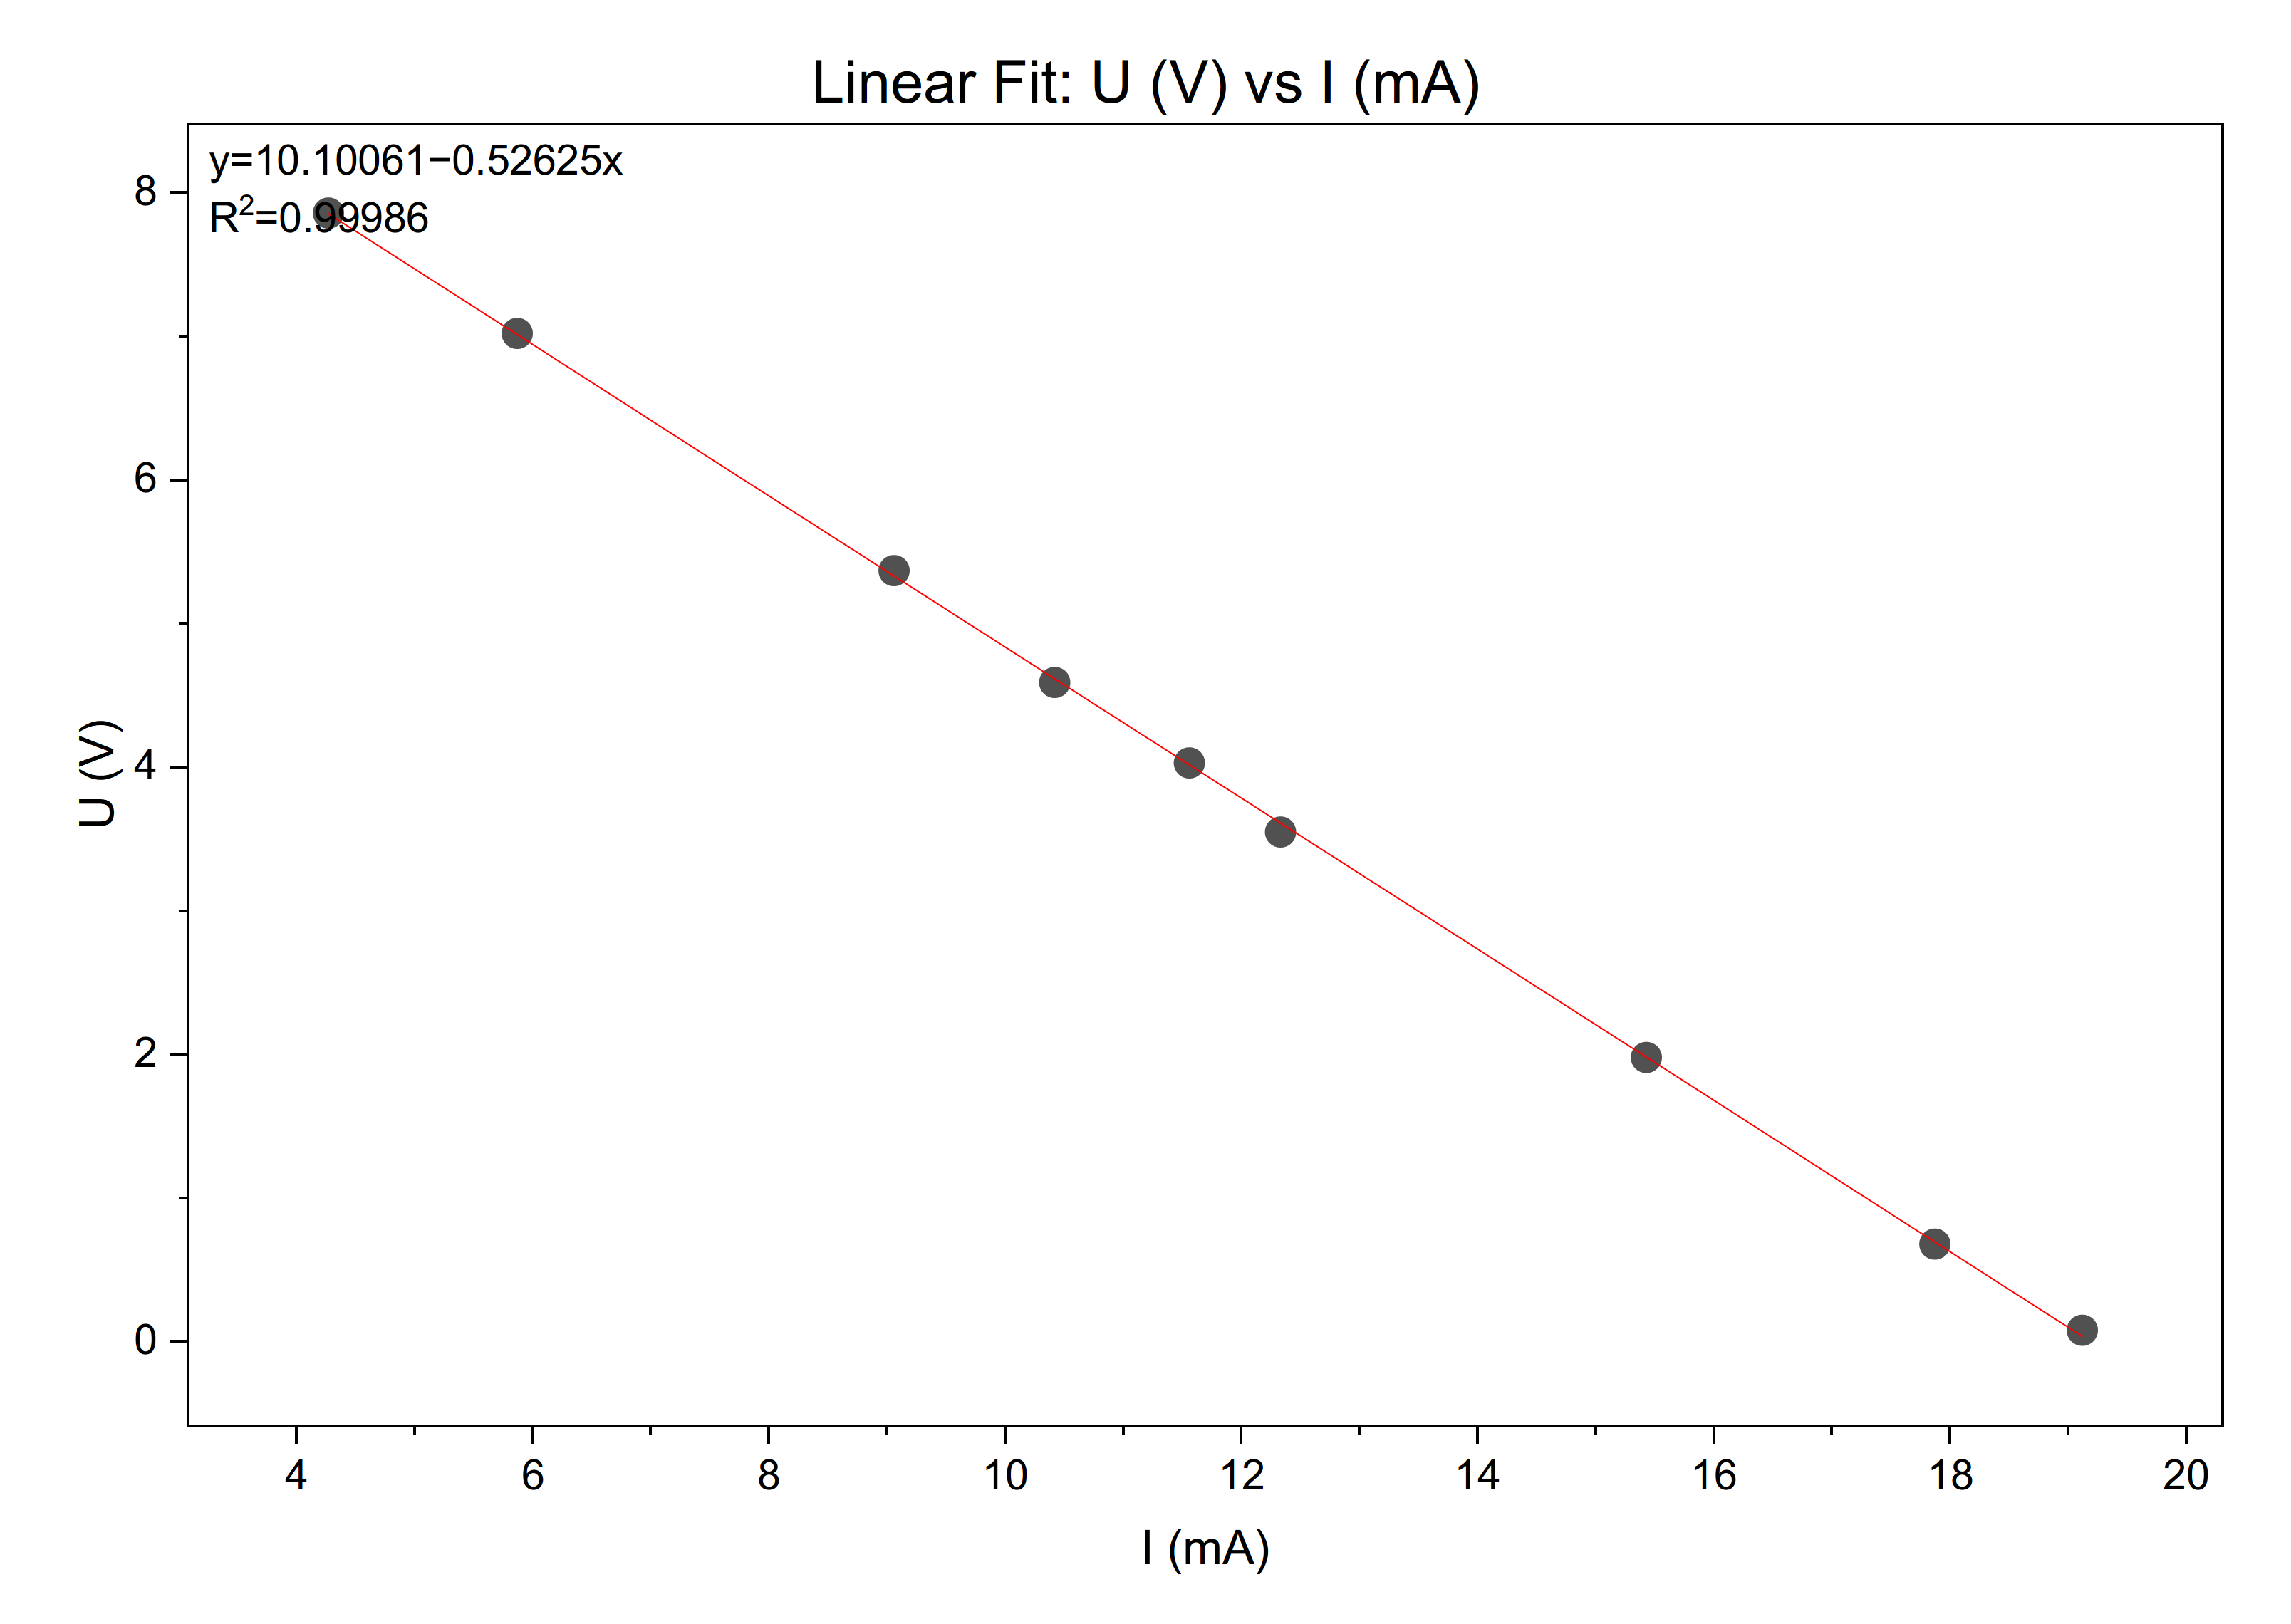
\includegraphics[width=\textwidth]{fig/Origin.png}
        \caption{原电路伏安特性曲线}
        \label{duoliangchengdianliu}
    \end{subfigure}
    \hfill
    \begin{subfigure}[b]{0.45\textwidth}
        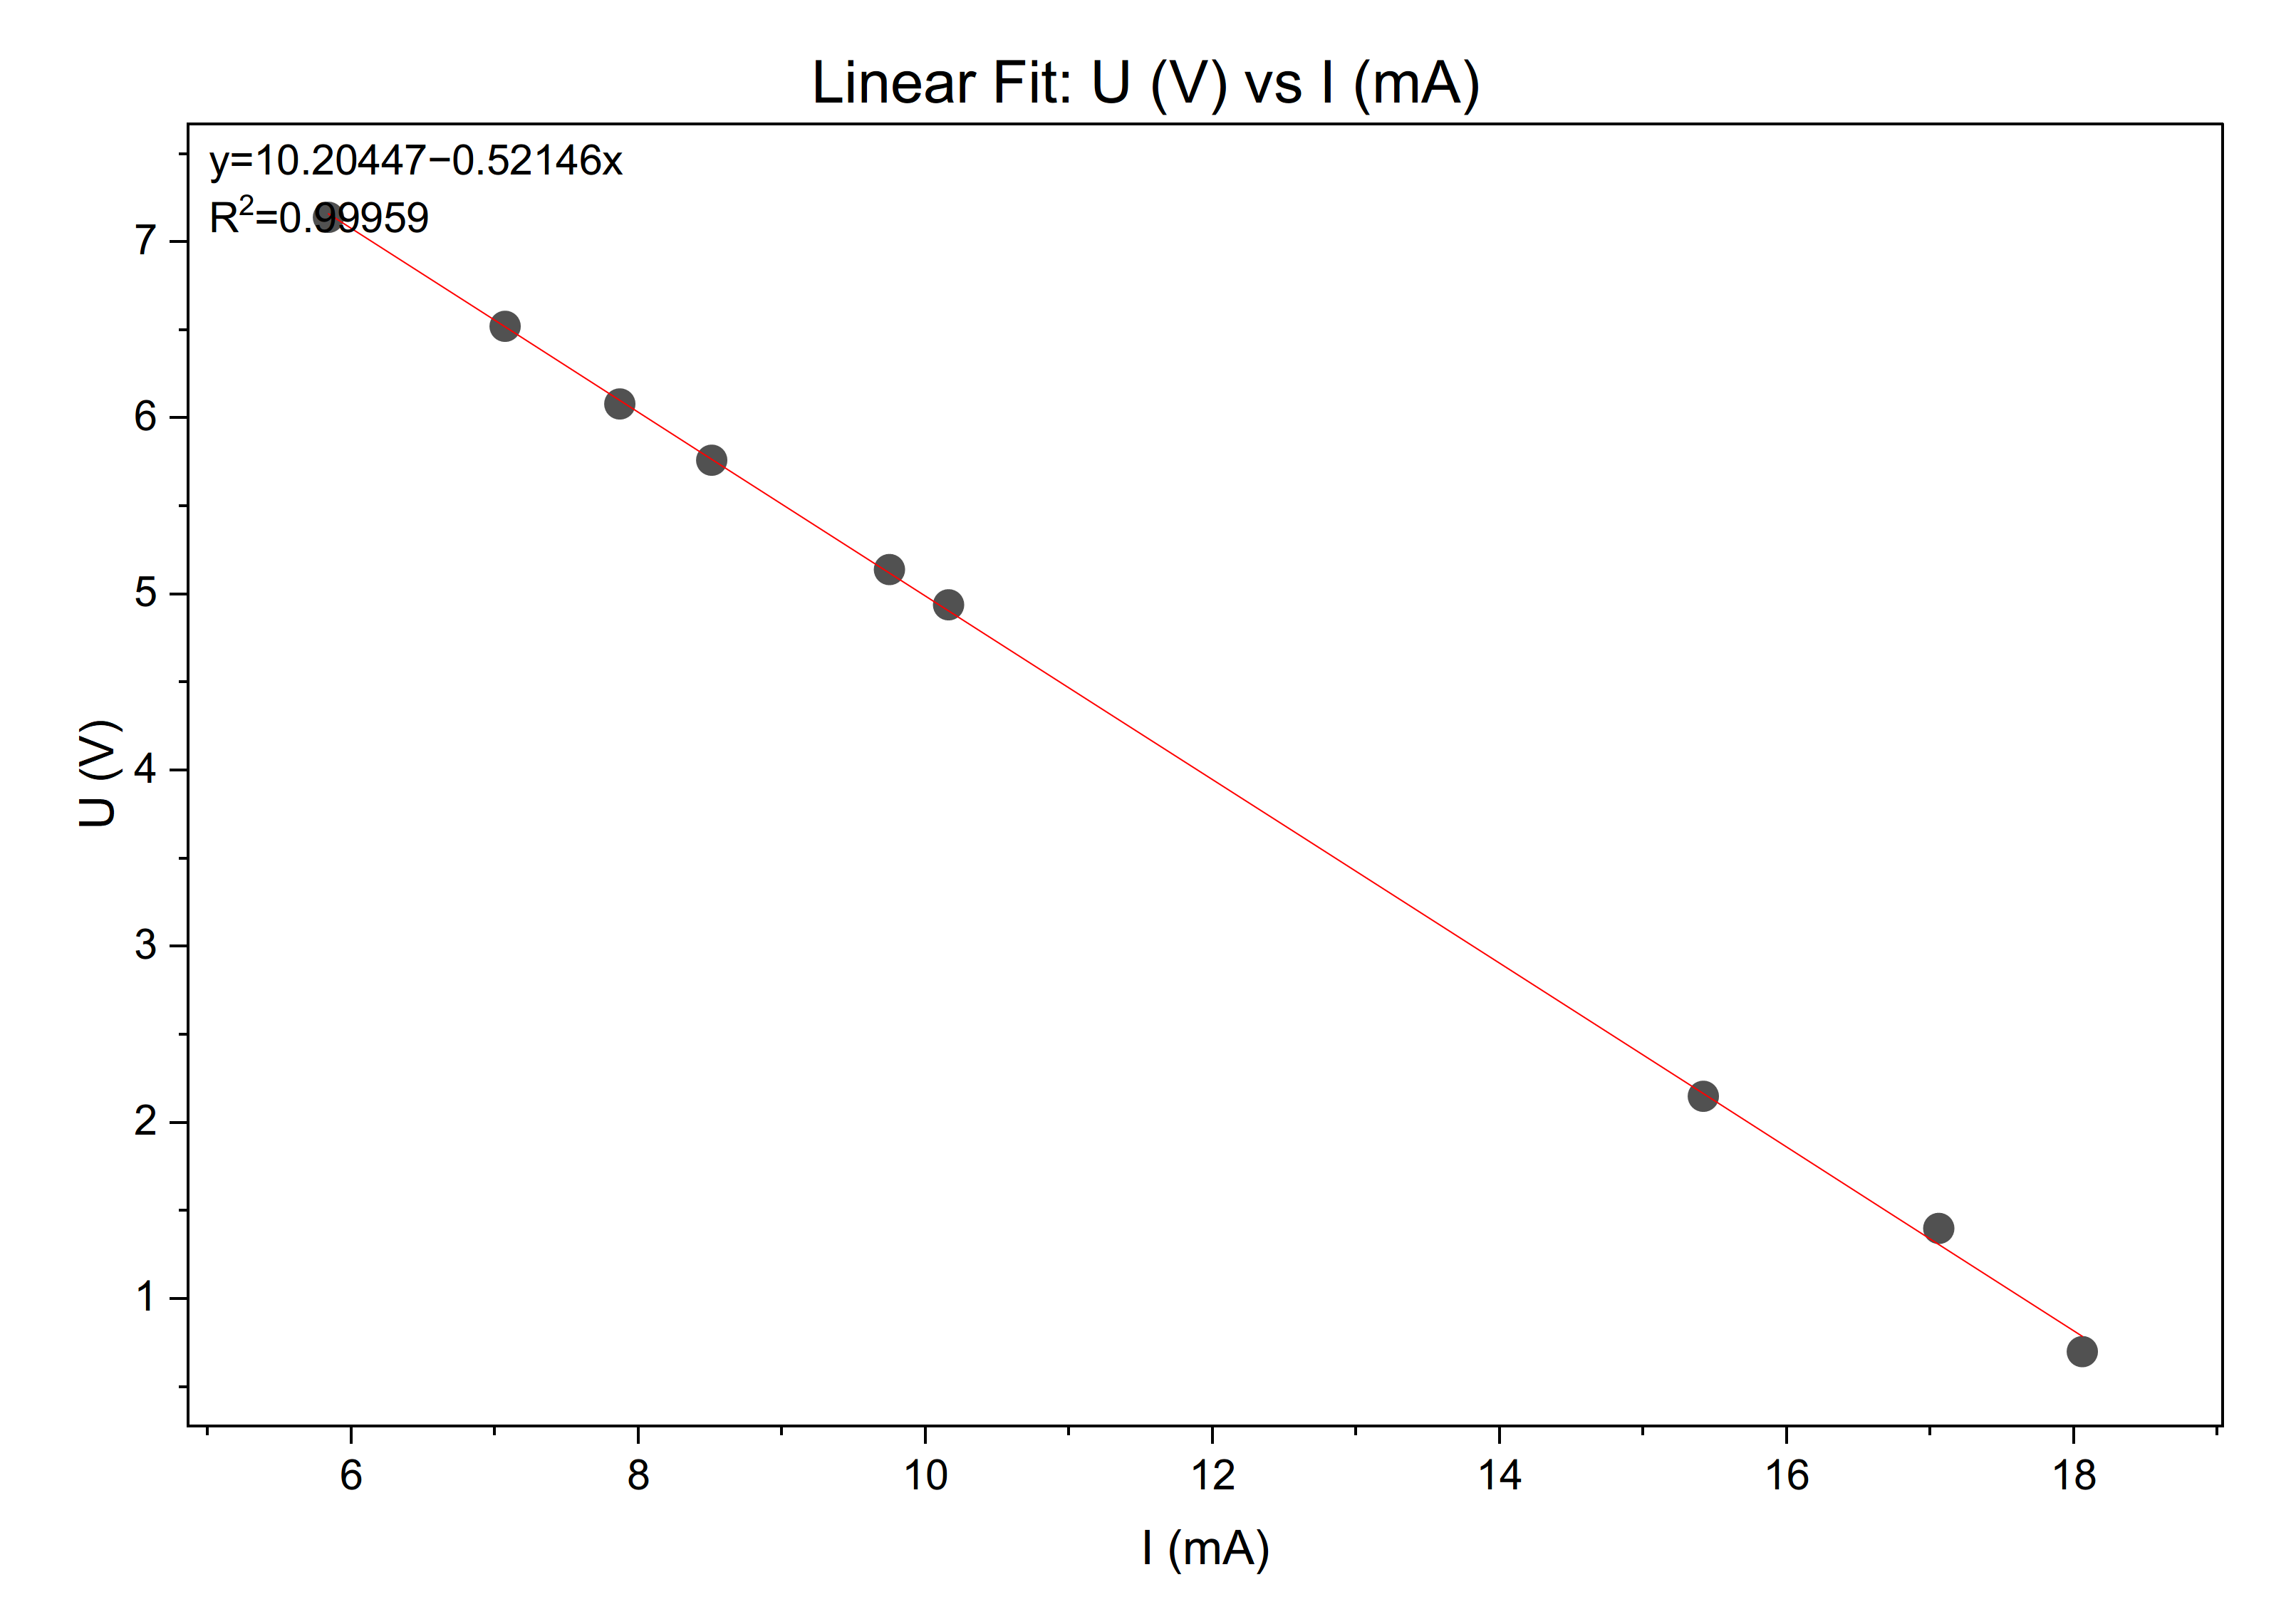
\includegraphics[width=\textwidth]{fig/戴维南等效数据.png}
        \caption{戴维南等效后的电路伏安特性曲线}
        \label{duoAjiaoyan}
    \end{subfigure}
    \caption{多量程电流表相关电路}
    \end{figure}

    从拟合结果可以看出，两者伏安特性曲线类似，可以说明该实验较为成功，而且验证了戴维南定理的正确性。
\section{结论}
可以使用戴维南定理代替一个有源二端口网络，获得与该网络相同的伏安特性曲线。

\section{心得与体会}
本次实验测试了很多测试点，锻炼了我的细心和耐心。

同时，本次实验中Origin拟合的应用，也展现了其作为现代化数据处理工具的强大效能，为高效分析实验数据提供了有力支持。
\section{思考题}
\subsection{在求戴维南或诺顿等效电路时，做短路实验，则测$I_{sc}$的条件是什么?}

在进行短路实验以测量 $I_{sc}$（诺顿等效电流）时，必须遵循以下两个关键条件：

\begin{itemize}
    \item \textbf{移除负载：}
    在测量 $I_{sc}$ 之前，必须首先将原先连接在AB端口上的任何外部负载（$R_L$）彻底断开，使测量点与原负载完全分离。

    \item \textbf{安全性评估：}
    必须确保网络的等效内阻（$R_{eq}$）具有足够大的值。这是为了防止在AB端口短路时，产生的短路电流 $I_{sc}$ 超过电源或电路内部元件所能承受的额定上限，从而避免烧毁器件。
\end{itemize}


\subsection{在本实验中可否直接做负载短路实验?}
\textbf{不可以。}
直接短路是一种高风险操作，它相当于接入了一个阻值极小（$R_L \approx 0$）的负载。

如果在执行短路前，没有对网络的开路电压 $U_{oc}$ 和等效内阻 $R_{eq}$ 有一个基本的估算，我们就无法预知短路电流 $I_{sc}$ 的大小。如果该网络的等效内阻 $R_{eq}$ 恰好非常小，那么 $I_{sc}$ 将会非常大，这极有可能瞬间导致电源过载或烧毁电路中的关键元件。
\subsection{简述测量有源二端口网络开路电压及等效内阻的几种方法，并比较其优缺点。}
在测定有源二端网络的开路电压及等效内阻时，常用的实验方法包括开路电压-短路电流法、伏安特性法和半电压法。这几种方法在操作、精度和适用性上各有不同。
\begin{itemize}
    \item \textbf{开路电压、短路电流法}

    这种方法通过分别测量网络开路时的电压（$U_{oc}$）和短路时的电流（$I_{sc}$），然后利用欧姆定律（$R_{eq} = U_{oc} / I_{sc}$）直接计算出等效内阻。

    \item \textbf{伏安特性法}

    这种方法是在网络两端接入可变负载，测量并记录多组对应的端电压 $U$ 和电流 $I$。然后通过绘制 $U-I$ 关系图线，根据图线的截距和斜率来确定开路电压和等效内阻。


    \item \textbf{半电压法}

    这种方法先测出开路电压 $U_{oc}$，然后接入一个电阻箱并调节其阻值 $R$，直到网络端电压恰好等于开路电压的一半（$U_{oc} / 2$）。此时，该电阻箱的读数 $R$ 即被视为等于等效内阻 $R_{eq}$。
\end{itemize}
\begin{table}[H]
    \centering
    \caption{三种测量方法的优缺点比较}
    \begin{tabularx}{\textwidth}{lXX}
        \toprule
        \textbf{测量方法} & \textbf{优点} & \textbf{缺点} \\
        \midrule
        \textbf{开路电压-短路电流法} &
        \begin{itemize}
            \item 测量方法简单，容易操作。
        \end{itemize} &
        \begin{itemize}
            \item 当网络内阻很小时，短路操作易导致电流过大，损坏内部元件。
        \end{itemize} \\
        \midrule
        \textbf{伏安特性法} &
        \begin{itemize}
            \item 利用伏安特性曲线可以直观地分析电压与电流的依赖关系。
        \end{itemize} &
        \begin{itemize}
            \item 需要进行多次测量并作图，过程比较繁琐。
            \item 当电表（尤其电流表）的内阻较大时，会引入显著的测量误差。
        \end{itemize} \\
        \midrule
        \textbf{半电压法} &
        \begin{itemize}
            \item 方法相对简单，可获得较高的测量精度，误差较小。
            \item 测量结果不受电源电压轻微波动的影响，稳定性好。
        \end{itemize} &
        \begin{itemize}
            \item 需要使用精度较高的电源和测量仪表。
            \item 测量和调节次数较多，相对复杂一些。
        \end{itemize} \\
        \bottomrule
    \end{tabularx}
\end{table}
\end{document}